%%%%%%%%%%%%%%%%%%%%%%%%%%%%%%%%%%%%%%%%%
% Beamer Presentation
% LaTeX Template
% Version 1.0 (10/11/12)
%
% This template has been downloaded from:
% http://www.LaTeXTemplates.com
%
% License:
% CC BY-NC-SA 3.0 (http://creativecommons.org/licenses/by-nc-sa/3.0/)
%
%%%%%%%%%%%%%%%%%%%%%%%%%%%%%%%%%%%%%%%%%

%----------------------------------------------------------------------------------------
%	PACKAGES AND THEMES
%----------------------------------------------------------------------------------------

\documentclass{beamer}

\mode<presentation> {

% The Beamer class comes with a number of default slide themes
% which change the colors and layouts of slides. Below this is a list
% of all the themes, uncomment each in turn to see what they look like.

%\usetheme{default}
%\usetheme{AnnArbor}
%\usetheme{Antibes}
%\usetheme{Bergen}
%\usetheme{Berkeley}
%\usetheme{Berlin}
\usetheme{Boadilla}
%\usetheme{CambridgeUS}
%\usetheme{Copenhagen}
%\usetheme{Darmstadt}
%\usetheme{Dresden}
%\usetheme{Frankfurt}
%\usetheme{Goettingen}
%\usetheme{Hannover}
%\usetheme{Ilmenau}
%\usetheme{JuanLesPins}
%\usetheme{Luebeck}
%%\usetheme{Madrid}
%\usetheme{Malmoe}
%\usetheme{Marburg}
%\usetheme{Montpellier}
%\usetheme{PaloAlto}
%\usetheme{Pittsburgh}
%\usetheme{Rochester}
%\usetheme{Singapore}
%\usetheme{Szeged}
%\usetheme{Warsaw}

% As well as themes, the Beamer class has a number of color themes
% for any slide theme. Uncomment each of these in turn to see how it
% changes the colors of your current slide theme.

%\usecolortheme{albatross}
%\usecolortheme{beaver}
%\usecolortheme{beetle}
%\usecolortheme{crane}
%\usecolortheme{dolphin}
%\usecolortheme{dove}
%\usecolortheme{fly}
%\usecolortheme{lily}
%\usecolortheme{orchid}
%\usecolortheme{rose}
%\usecolortheme{seagull}
\usecolortheme{seahorse}
%\usecolortheme{whale}
%\usecolortheme{wolverine}

%\setbeamertemplate{footline} % To remove the footer line in all slides uncomment this line
%\setbeamertemplate{footline}[page number] % To replace the footer line in all slides with a simple slide count uncomment this line

%\setbeamertemplate{navigation symbols}{} % To remove the navigation symbols from the bottom of all slides uncomment this line
}

\usepackage{graphicx} % Allows including images
\usepackage{booktabs}
\usepackage{movie15} % Allows the use of \toprule, \midrule and \bottomrule in tables

%----------------------------------------------------------------------------------------
%	TITLE PAGE
%----------------------------------------------------------------------------------------
\setbeamertemplate{navigation symbols}{} %turn off navigation symbols
\title[URM]{Umbilical Retrieval Mechanism (URM) Update} % The short title appears at the bottom of every slide, the full title is only on the title page

\author{Jerin Roberts} % Your name

\institute[TRU] % Your institution as it will appear on the bottom of every slide, may be shorthand to save space
{
 
\textit{robertsj@snolab.ca} \\

}
\date{\today} % Date, can be changed to a custom date

\begin{document}

\begin{frame}
\centering

\includegraphics[width=0.15\linewidth]{tru}
\titlepage % Print the title page as the first slide
\end{frame}

\begin{frame}
\frametitle{Overview} % Table of contents slide, comment this block out to remove it
\tableofcontents % Throughout your presentation, if you choose to use \section{} and \subsection{} commands, these will automatically be printed on this slide as an overview of your presentation
\end{frame}

%----------------------------------------------------------------------------------------
%	PRESENTATION SLIDES
%----------------------------------------------------------------------------------------

%------------------------------------------------
\section{General Overview} % Sections can be created in order to organize your presentation into discrete blocks, all sections and subsections are automatically printed in the table of contents as an overview of the talk
%------------------------------------------------

\subsection{Modifications} % A subsection can be created just before a set of slides with a common theme to further break down your presentation into chunks


\begin{frame}
\frametitle{URM Function}
Controls the deployment and storage of the source umbilical for the SNO+ detector\\~\\
\centering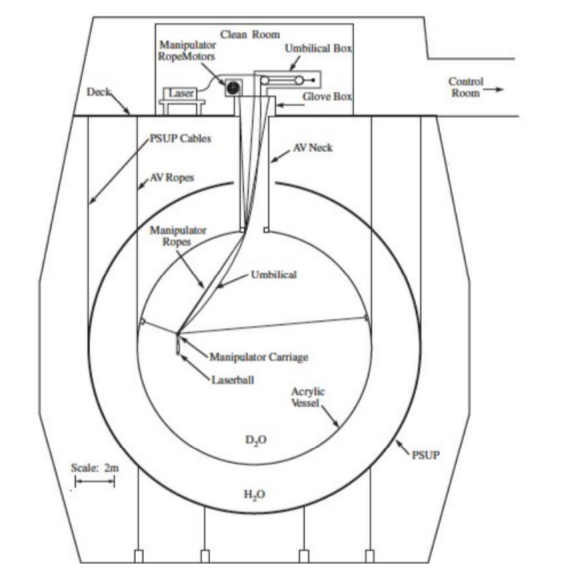
\includegraphics[width=0.5\linewidth]{avdia}
\centering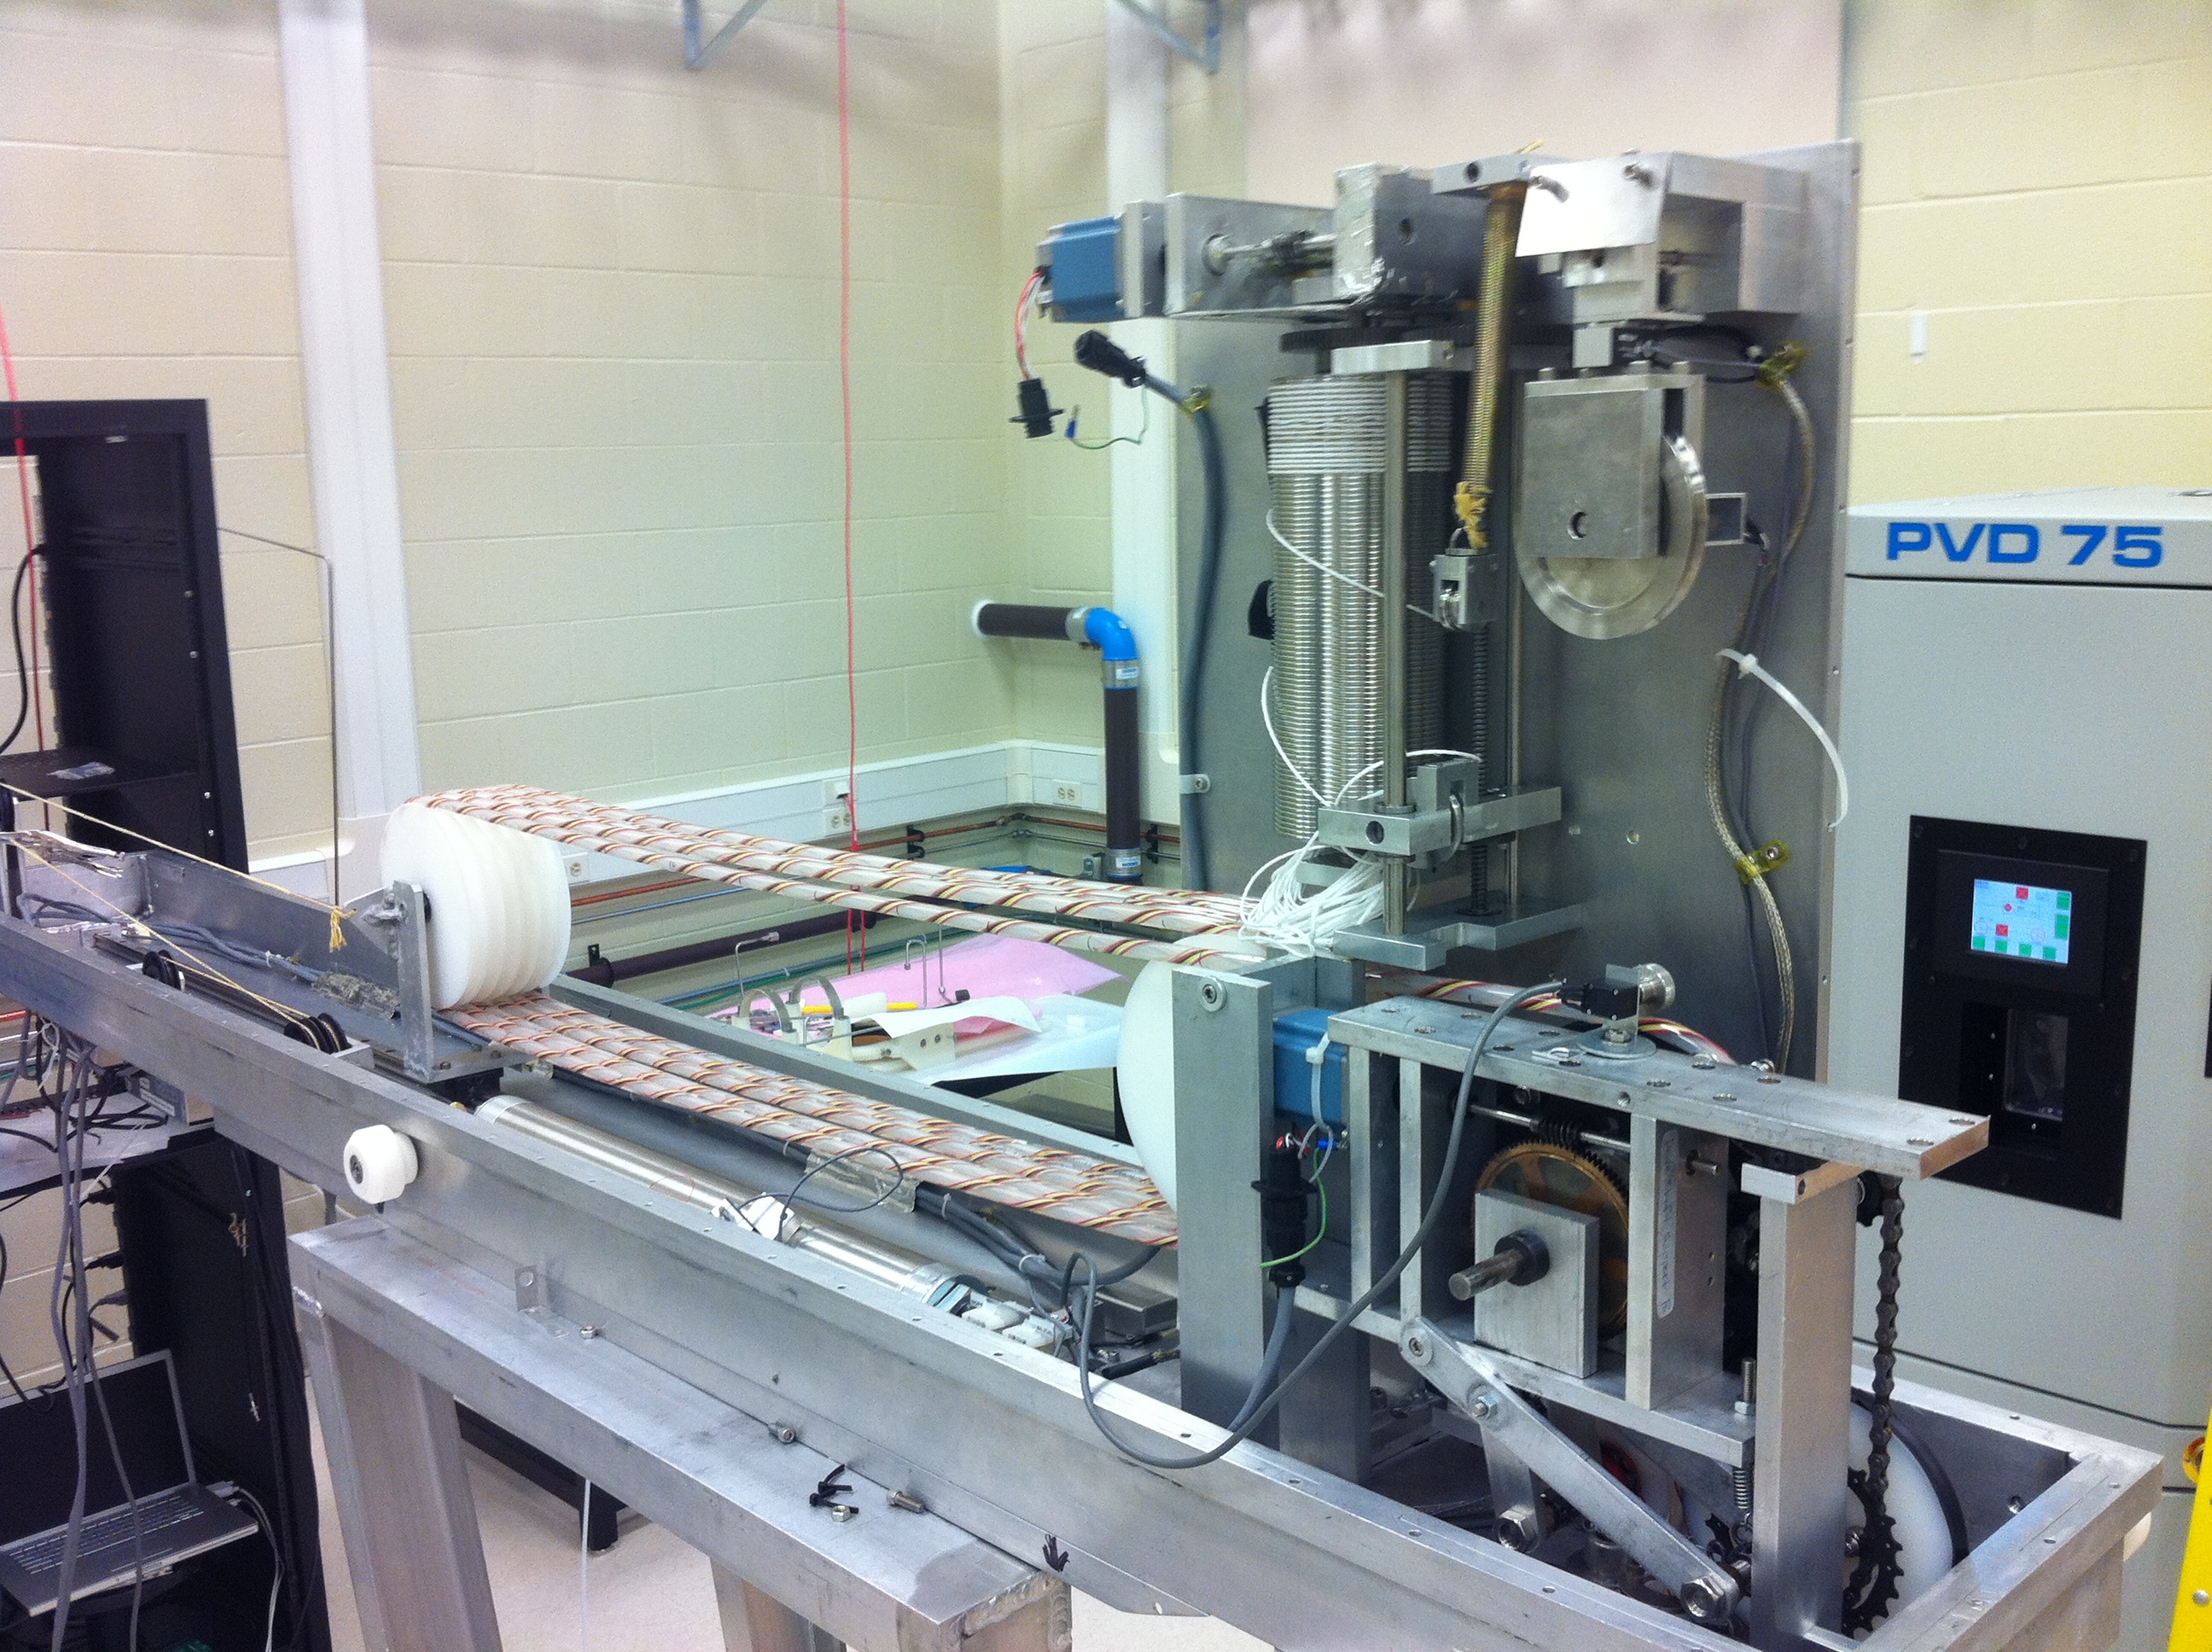
\includegraphics[width=0.5\linewidth]{IMG_1204}
\end{frame}

%------------------------------------------------
\subsection{Internal Structure}
\begin{frame}
\frametitle{How it Works}
\centering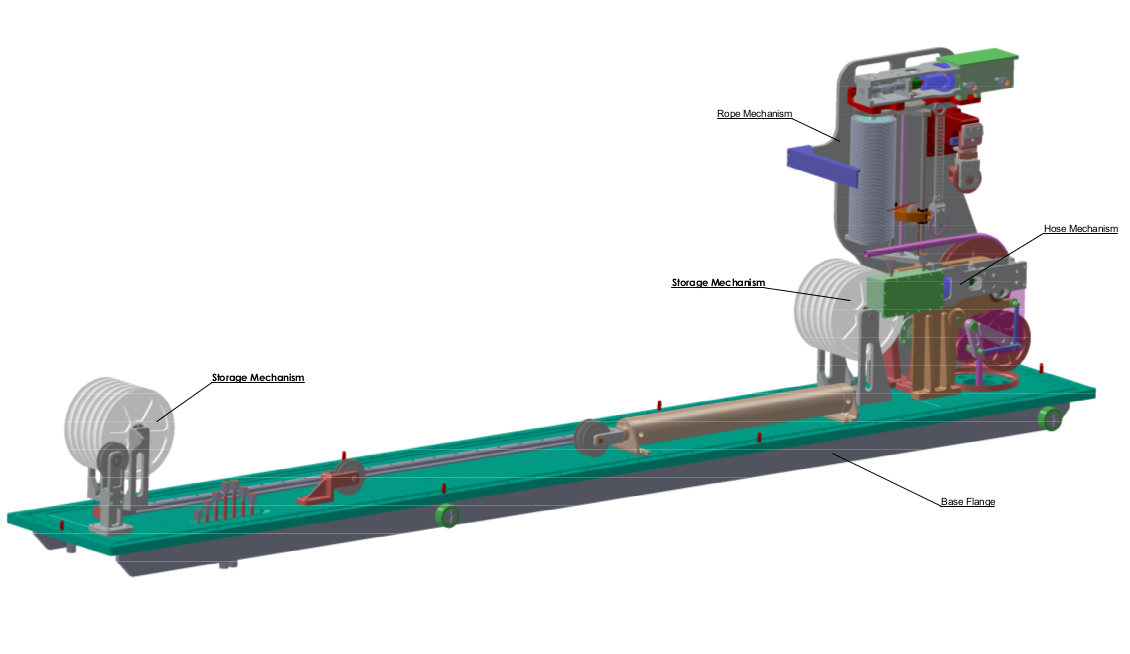
\includegraphics[width=1\linewidth]{scehm}
\end{frame}
\begin{frame}
\frametitle{Drive Pulley Assembly Before:}
The drive pulley assembly extends and retracts the umbilical \\~\\
\centering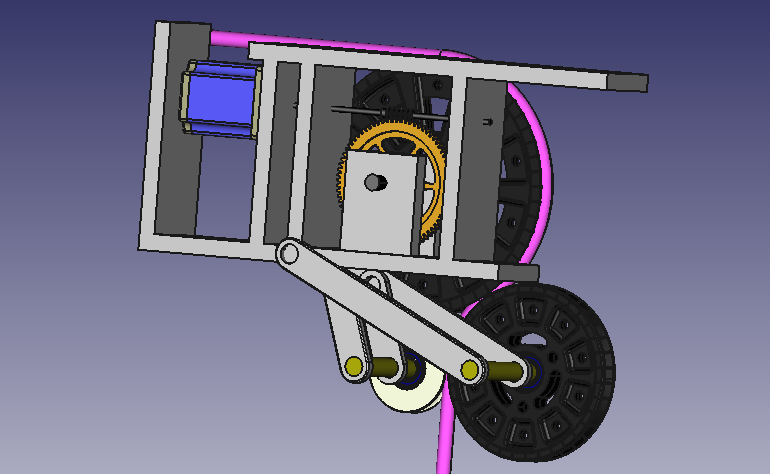
\includegraphics[trim = 20mm 0mm 20mm 0mm, height=3.5cm]{original1}
\centering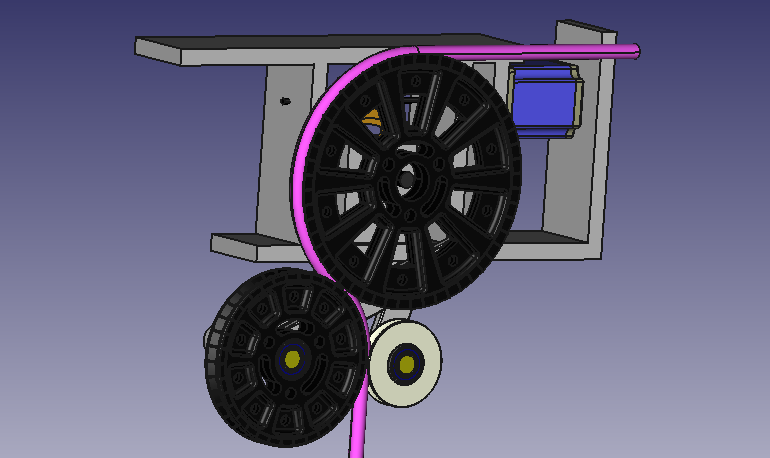
\includegraphics[trim = 20mm 0mm 20mm 0mm, height=3.5cm]{original2}
\end{frame}

\subsection{Problems}

\begin{frame}
\frametitle{URM Problems}
\begin{columns}[t] % The "c" option specifies centered vertical alignment while the "t" option is used for top vertical alignment

\column{1\textwidth} % Left column and width
\textbf{Sources of Slippage:}
\begin{enumerate}
\item LAB as Scintillator (low coefficient of friction)
\item LAB and Water compatible umbilical
\item Pulley Design (collects LAB reducing friction)
\item Umbilical Storage System (Pneumatic Cylinder)
\end{enumerate}



\end{columns}
\end{frame}


%------------------------------------------------
\subsection{Chain Drive Design}
\begin{frame}
\frametitle{The Drive Pulley Design}
\centering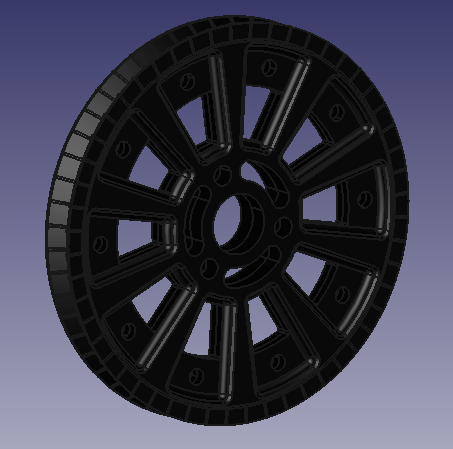
\includegraphics[height=2.5cm]{pull1}
\centering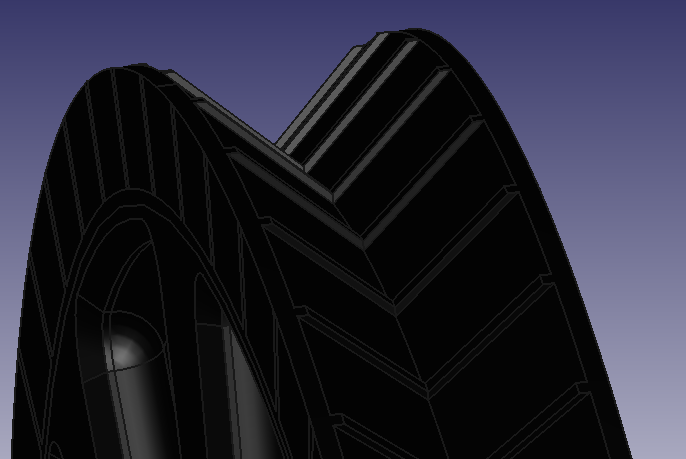
\includegraphics[height=2.5cm]{pull3} \\
\centering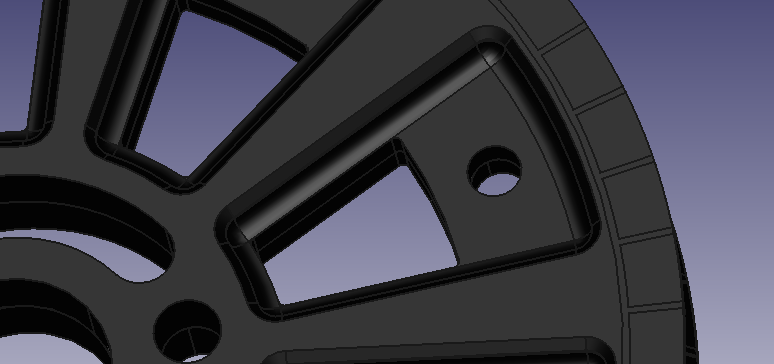
\includegraphics[height=2.95cm]{pull2}

\end{frame}
\begin{frame}
\frametitle{Chain Drive Design}
\centering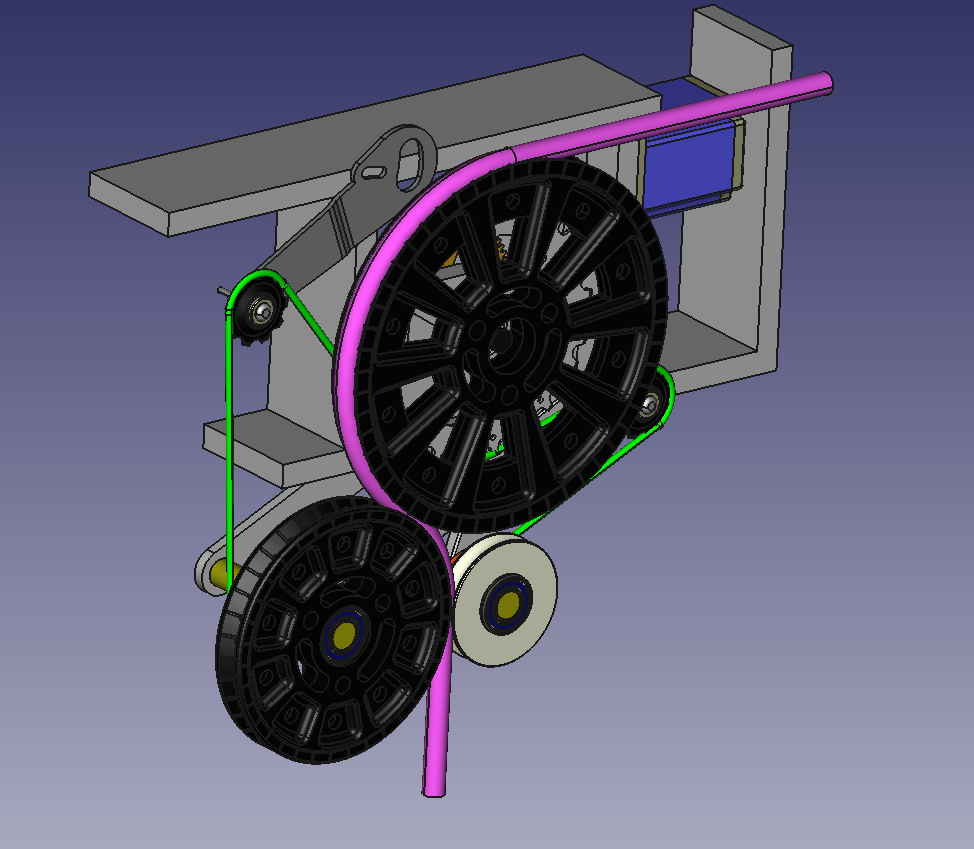
\includegraphics[height=4cm]{final1}
\centering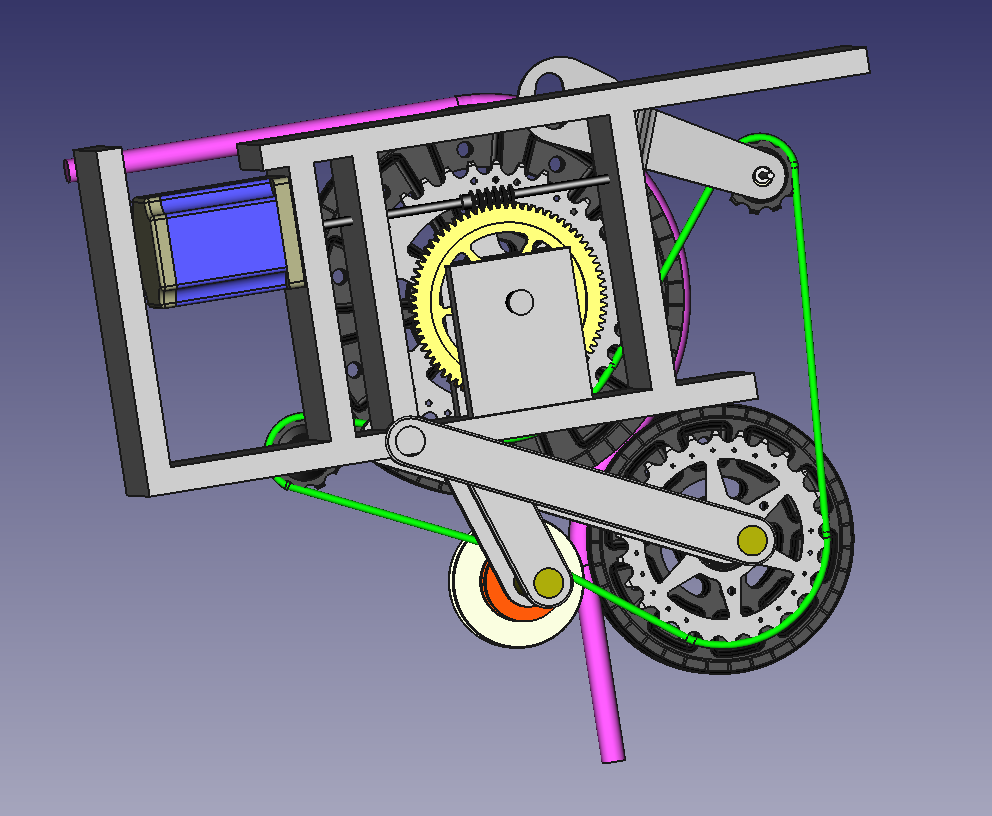
\includegraphics[height=4cm]{final2}
\end{frame}
\begin{frame}
\frametitle{Chain Drive Design}
\centering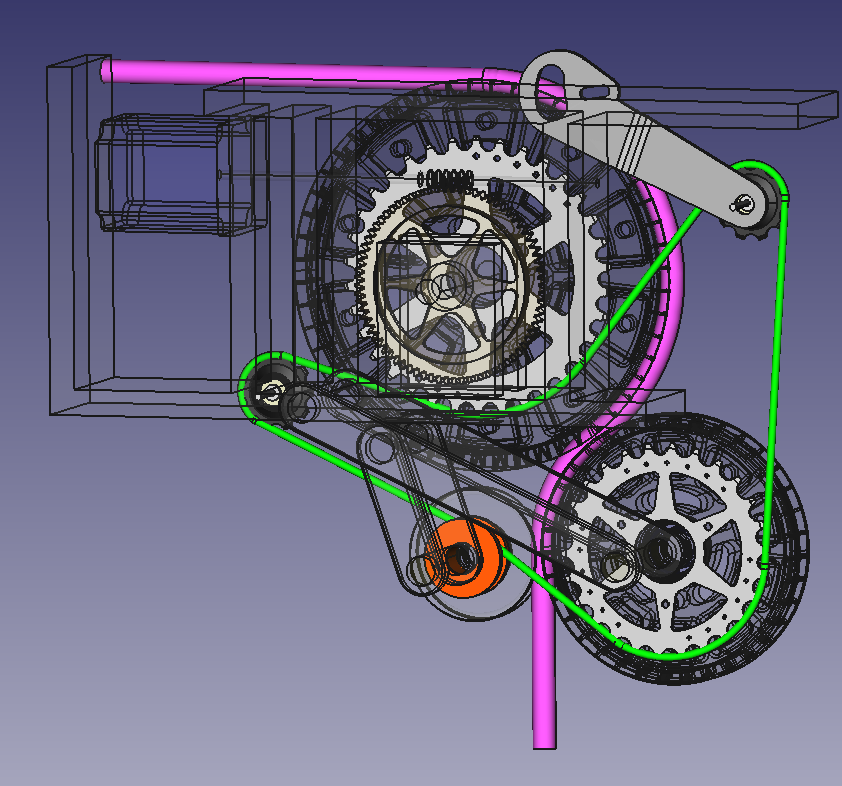
\includegraphics[height=4cm]{final3}
\centering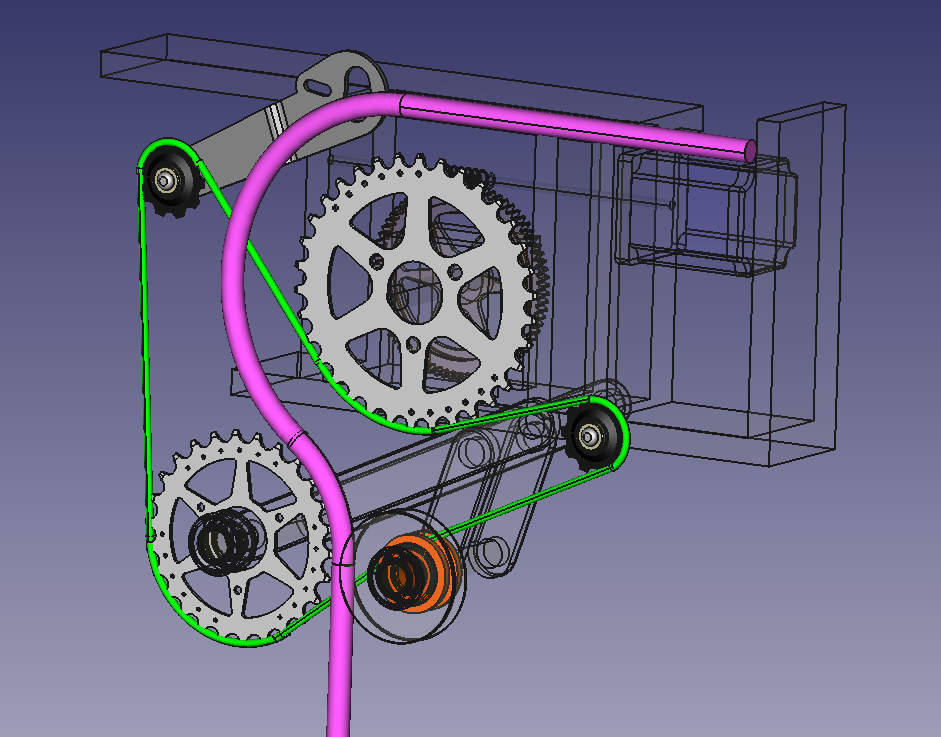
\includegraphics[height=4cm]{final4}
\end{frame}

\section{Performance}
%------------------------------------------------
\subsection{Data}


\begin{frame}
\frametitle{Chain Drive vs Non-chain drive}
\centering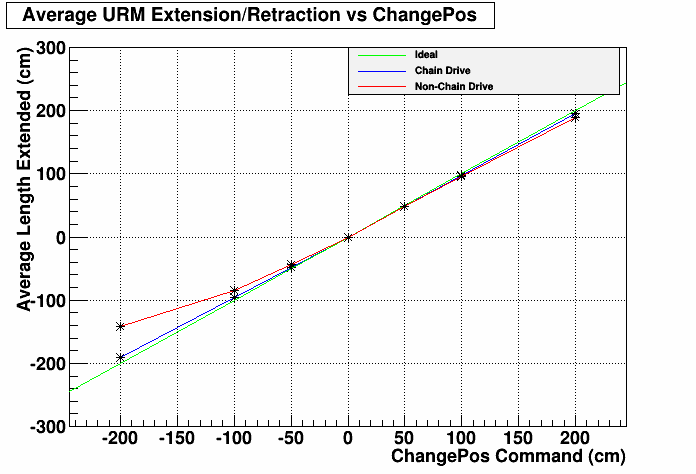
\includegraphics[width=8cm]{Newumb1.png}
\end{frame}

\begin{frame}
\frametitle{Chain Drive Fit}
\centering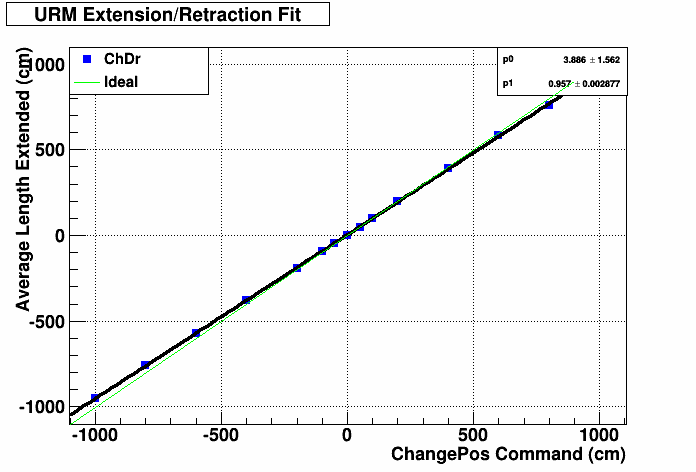
\includegraphics[width=8cm]{FIT1.png}
\end{frame}
\begin{frame}
\frametitle{Chain Drive Consistency}
\centering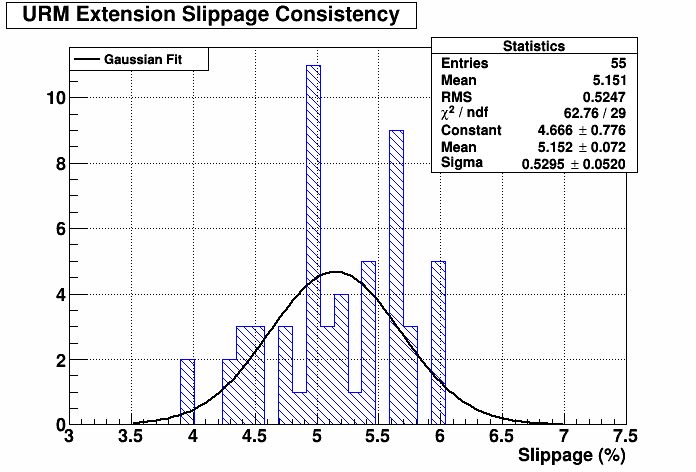
\includegraphics[width=6cm]{Hist1.png}
\centering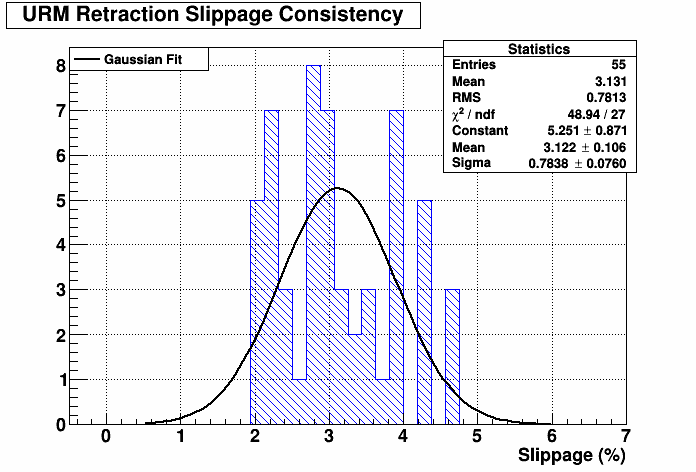
\includegraphics[width=6cm]{Hist2.png}
\end{frame}
\begin{frame}
\frametitle{Non-Chain Drive Consistency}
\centering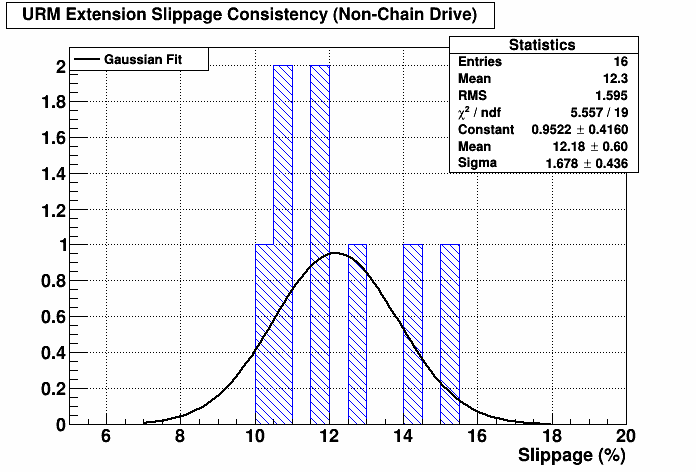
\includegraphics[width=6cm]{Hist5.png}
\centering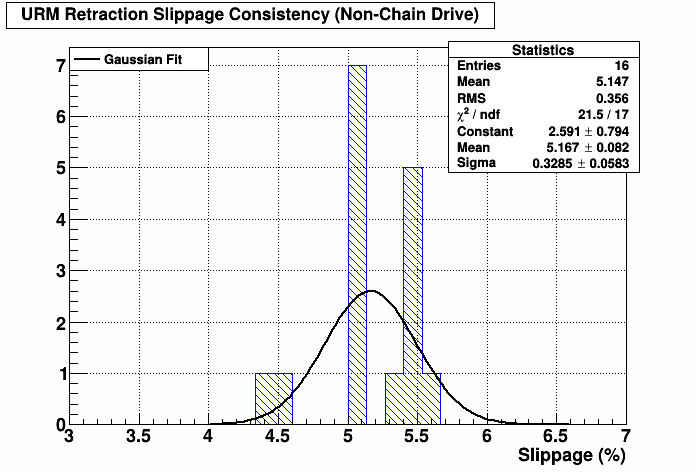
\includegraphics[width=6cm]{Hist6.png}
\end{frame}
\begin{frame}
\frametitle{Chain Drive Consistency}
\centering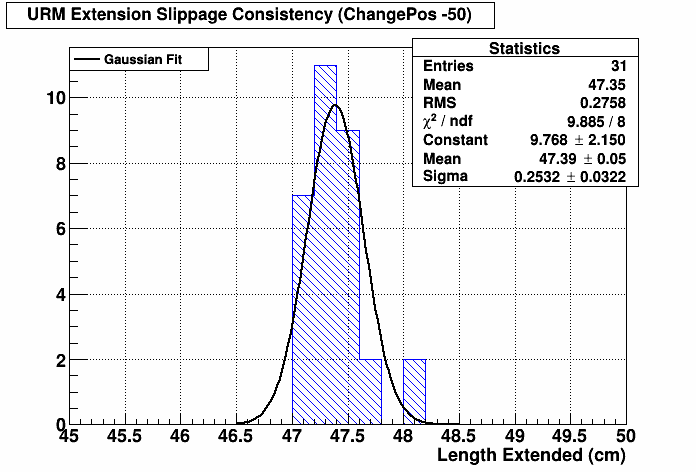
\includegraphics[width=6cm]{Hist3.png}
\centering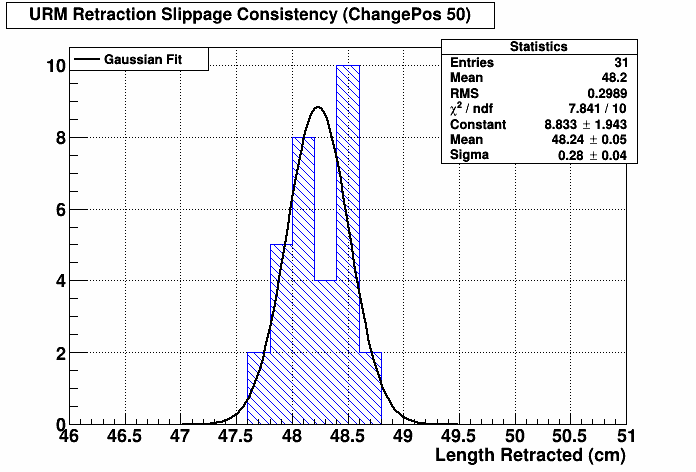
\includegraphics[width=6cm]{Hist4.png}
\end{frame}


\subsection{Implementation}

\begin{frame}
\frametitle{New URM Design}
\centering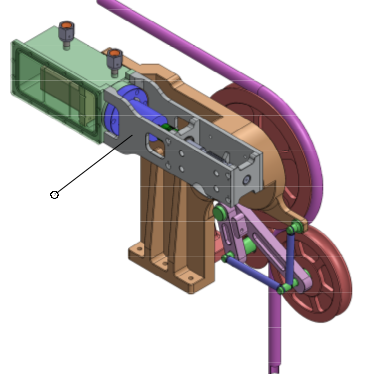
\includegraphics[width=5cm]{newsch1.png}
\centering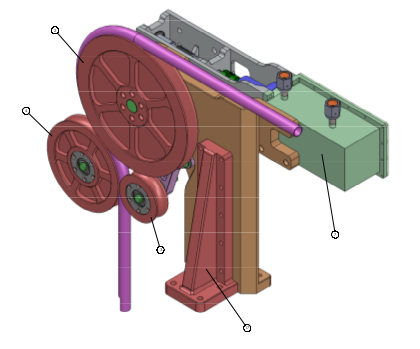
\includegraphics[width=5cm]{newsch2.png}
\end{frame}

\begin{frame}
\frametitle{Flex Drive}
\centering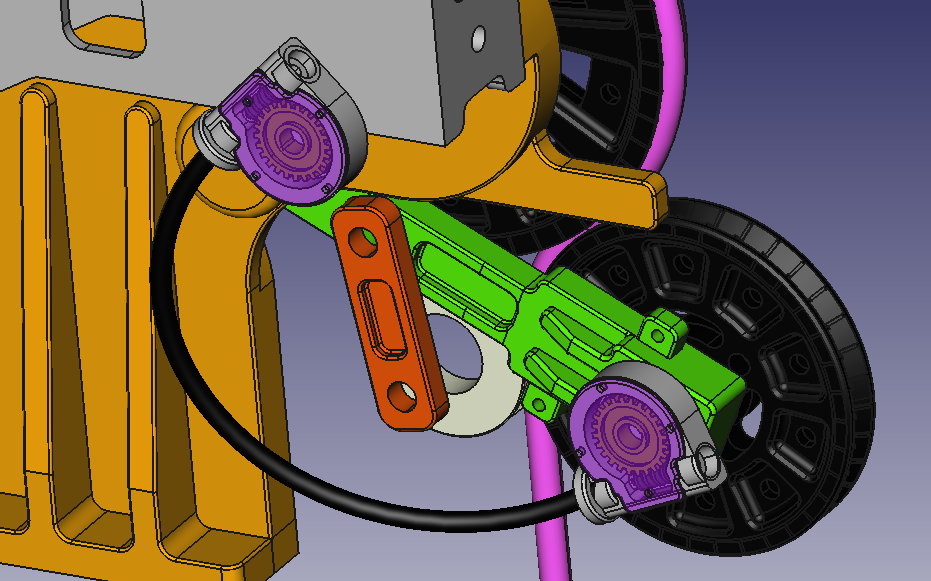
\includegraphics[width=10cm]{newurm1.png}
\end{frame}

\begin{frame}
\frametitle{Flex Drive}
\centering
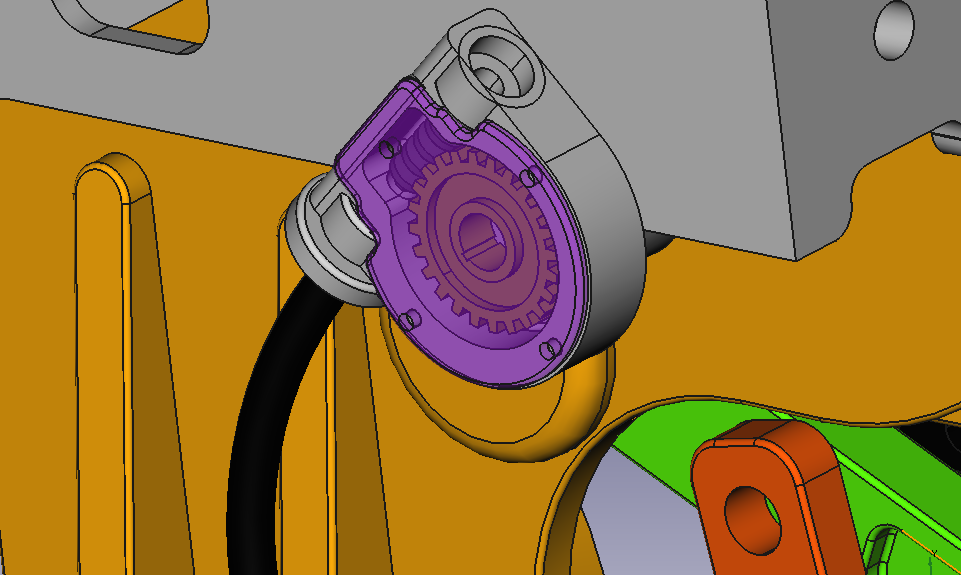
\includegraphics[width=10cm]{newurm3.png}
\end{frame}

\begin{frame}
\frametitle{Chain/Gear Drive}
\centering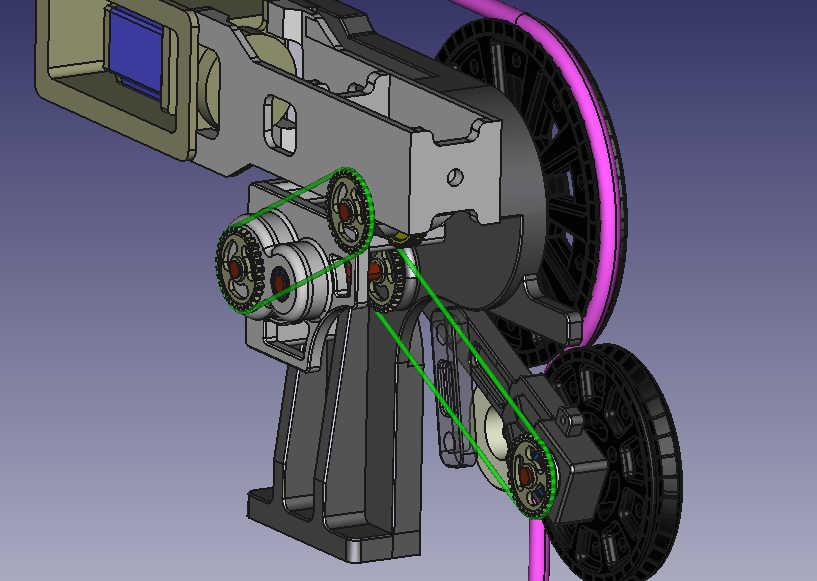
\includegraphics[width=10cm]{URM1.png}
\end{frame}

\begin{frame}
\frametitle{Chain/Gear Drive}
\centering
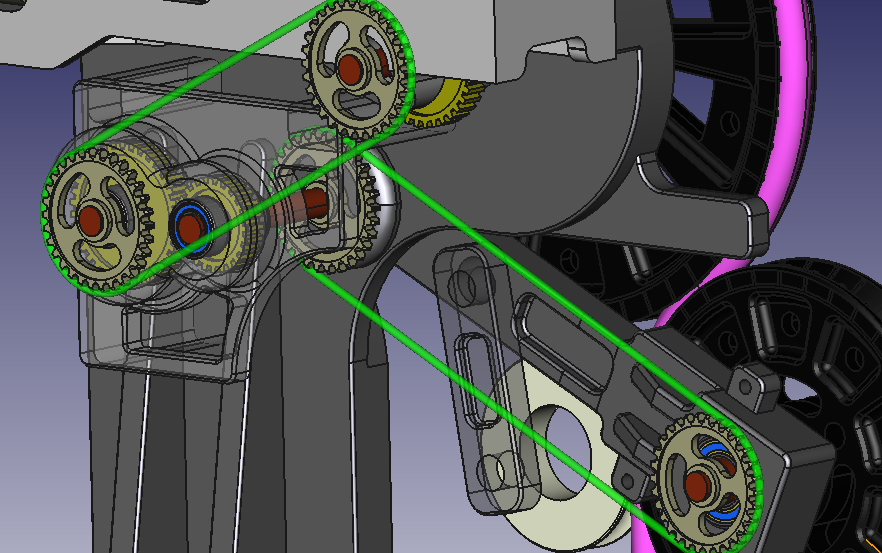
\includegraphics[width=10cm]{URM2.png}
\end{frame}
%------------------------------------------------

\section{Future Goals}
\subsection{Next Steps}

\begin{frame}
\frametitle{Future Goals}
\begin{columns}[t] % The "c" option specifies centered vertical alignment while the "t" option is used for top vertical alignment

\column{1\textwidth} % Left column and width
\textbf{Next Steps:}
\begin{enumerate}
\item Determine Consistency of Chain Drive system
\item Investigate the possible Improvements of driving small pulley
\item Complete LAB application system
\item Investigate Implementing Drive System to new URM design
\end{enumerate}



\end{columns}

\end{frame}

%------------------------------------------------


\begin{frame}
\frametitle{References}
\footnotesize{
\begin{thebibliography}{99} % Beamer does not support BibTeX so references must be inserted manually as below
\bibitem[Garcia, 2014]{p1} Lawrence Garcia (2014)
\newblock Umbilical Tests and Detector Data Analysis


\bibitem[Smith, 2013]{p1} Jose Maneira, Rui Alves (2013)
\newblock URM design for SNO+, LIP-Coimbra

\end{thebibliography}
}
\end{frame}

%------------------------------------------------

\begin{frame}
\Huge{\centerline{Thank-you}}
\end{frame}

%----------------------------------------------------------------------------------------

\end{document} 